\documentclass[12pt]{article}


\usepackage[utf8]{inputenc}
\usepackage[T1]{fontenc}
\usepackage[francais]{babel}
\usepackage{hyperref}
\usepackage{pifont}
\usepackage{algorithmic}
\usepackage{algorithm}
\usepackage{graphicx}

\title{Projet réseau - Chat Python}
\author{Loïc Lachiver}
\author{Romain Pigret-Cadou}

\begin{document}
\maketitle


\begin{abstract}
    \begin{center}
    \url{https://github.com/picachoc/IRC_python}
    \\Projet UE Réseau L2
    \\Université de Bordeaux
    \\Groupe TMA12\_13
    \\Année 2019
    \end{center}
\end{abstract}


\tableofcontents



\section{Introduction}
Dans le cadre de l'UE Réseau de la L2 informatique de l'Université de Bordeaux,
nous devions, pour nous initier aux sockets, réaliser un chat textuel en Python.
En s'inspirant fortement du protocole IRC, les fonctionnalités du chat nous étaient
imposées en 2 versions (0 et 1) via le cahier des charges disponible en Annexe.

\section{Fonctionnement général}

Deux scripts python sont donc nécessaires, le \textbf{client} et
le \textbf{serveur} (respectivement
client.py et server.py). Python a été préféré à d'autres langages pour sa simplicité
d'implémentation, il est vrai qu'il a été simple de mettre en place
certaines structures.

\underline{Le Serveur} a pour rôle d'orchestrer les différentes demandes des clients,
transmises par sockets. Il stocke aussi toutes les informations nécessaires comme
les canaux de discussion, les noms d'utilisateurs, qui est situé où, qui est admin, ...
Ces informations sont manipulées sous la forme de chaînes de caractères.
Pour communiquer avec le serveur il faut lui envoyer des commandes spécifiques,
de même il vous transmet ses informations via des commandes aussi (souvent le même intitulé).
En conséquence, pour se mettre d'accord sur ces commandes nous devions créer notre propre
protocole de communication \emph{(client <-> serveur)}.

\underline{Le Client} lui peut prendre diverse formes, que ce soit une application graphique
ou dans un terminal. L'intérêt du client est d'interpréter les commandes du protocole serveur
et de convertir en protocole serveur les ordres donnés par l'utilisateur, que se soit par un
clic sur un bouton ou en tapant "/commande". En effet le serveur est conçu pour fonctionner
parfaitement avec son protocole, d'ailleurs nous le testions avec la commande linux \emph{nc}.
Mais le client permet de rajouter une surcouche ergonomique, en traduisant les codes d'erreurs,
en parlant dans la langue utilisateur (français) et de manière plus claire que le protocole.

La conception du protocole serveur était totalement libre, seule la syntaxe et
la fonctionnalité des commandes
à taper dans le terminal client étaient imposées.


\section{Serveur}
Notre serveur est basé sur le protocole PICROM, intitulé par concaténation des
3 premières lettres de nos pseudonymes respectifs.

\subsection{Documentation}
Le serveur peut-être lancé UNIQUEMENT depuis un terminal linux avec
la commande : \emph{python3 server.py}
\\ou \emph{python3 server.py port} , sinon le port par défaut est 1459
\\

\noindent{\textbf{\underline{Protocole Client -> Serveur :}}}
\\

\noindent{\underline{Légende:}}
\\\ding{88} : Nécessite les droits administrateurs
\\\ding{108} : Le client ne peut l'utiliser que dans un $channel$ (canal de discussion)
\\\ding{110} : Utilisable uniquement en dehors de tout $channel$, dans le $HUB$
\\\ding{115} : Utilisable de n'importe où

\begin{description}
    \item[---LIST]:\ding{115} le client demande la liste des $channels$ ouverts
    \item[---JOIN <channelName>]:\ding{115} le client veut rejoindre le canal "channelName" 
    \item[---LEAVE]:\ding{108} le client veut quitter le $channel$
    \item[---WHO] :\ding{108} le client veut la liste des $nicks$(pseudonymes) des clients
    sur le $channel$ courant
    \item[---MSG <message>]:\ding{108} le client veut envoyer un message sur le $channel$
    \item[---PRV\_MSG N <nick1> ... <nickN> <message>]:\ding{108} le client veut
         envoyer un message privé à N utilisateurs identifiés par leurs $nicks$
    \item[---BYE]:\ding{110} le client veut se déconnecter du serveur
    \item[---KICK <nick>] \ding{88}\ding{108} l'administrateur veut $kicker$ nick
    du $channel$: lui forcer le LEAVE
    \item[---REN <newChannelName>] \ding{88}\ding{108} l'administrateur veut renommer le $channel$
    \item[---CURRENT <newChannel |>] \ding{115} le client veut définir un autre
    $channel$ préalablement JOIN comme son $channel$ courant | ou simplement
    demander son $channel$ courant
    \item[---NICK <newNick>] \ding{115} le client veut changer son pseudo
    \item[---GRANT <newAdminNick>] \ding{88}\ding{108} l'administrateur veut rendre admin
                                                un client sur le $channel$ 
    \item[---REVOKE <oldAdminNick>] \ding{88}\ding{108} l'administrateur veut destituer 
                                            un admin sur le $channel$
    \item[---SEND <nick> <file\_name>] \ding{108} demande d'envoi de fichier au serveur, à destination de nick
    \item[---SENDF <package> | void ] \ding{108} envoi d'une partie du fichier | SENDF seul pour indiquer la fin de la transmission
    \item[---RECV] \ding{108} demande de réception d'un fichier qui nous est destiné.
    \item[---RECVF] \ding{108} paquet bien reçu, demande du paquet suivant
    \\
\end{description}



\noindent{\textbf{\underline{Protocole Serveur -> Client :}}}
\\

\noindent{\underline{Légende:}}
\\<R> :  rang du client, 1 pour administrateur, 0 sinon
\\\ding{108} : Commande envoyée au client
\\\ding{110} : Commande envoyée aux autres clients du $channel$
\\\ding{115} : Commande envoyée à tout les autres clients du serveur
\\\ding{54} : Commande envoyée aussi au client"
\\\ding{88} : Commande envoyée au(x) client(s) cible(s)

\begin{description}
    \item[---ERR <code>] \ding{108} envoie d'un code d'erreur
    \item[---CONNECT <firstNick>] \ding{115}\ding{54} confirme la connexion
                                                        d'un nouveau client
    \item[---LIST <channel1> ... <channelN>] \ding{108} envoie la liste des $channels$
                                                ouverts, séparés par des espaces
    \item[---JOIN <channel> <R> <newCommerNick>] \ding{110}\ding{54} indique l'entrée
                                d'un nouveau client sur le $channel$, si votre rang est
                                1 alors vous venez d'ouvrir le $channel$
    \item[---LEAVE <channel> 0 <nick> | <channel> 1 <nick> <newAdmin>] \ding{110}\ding{54}
                indique qu'un client a quitté le $channel$ | indique un nouvel admin
                s'il était le dernier.
    \item[---WHO <R> <client1> ... <R> <clientN>] \ding{108} envoie la liste des clients
                                    sur le channel
    \item[---MSG <channel> <R> <nick> <message>] \ding{110} nick a envoyé un message sur le channel
    \item[---PRV\_MSG <channel> <R> <nick> <message>] \ding{88} nick vous a envoyé un message privé
    \item[---BYE <nick>] \ding{115} indique qu'un client s'est déconnecté du serveur
    \item[---KICK <channel> <adminNick> <R> <nick>] \ding{110}\ding{54} indique que nick va être
    immédiatement $kické$ par l'admin du $channel$
    \item[---REN <channel> <adminNick> <newName>] \ding{110}\ding{54} le $channel$ a été renommé par l'admin
    \item[---CURRENT <currentChannel>] \ding{108} indique au client son $channel$ courant ou celui qu'il vient de définir
    \item[---GRANT <channel> <adminNick> <newAdmin>] \ding{110}\ding{54} newAdmin a été promu admin par adminNick dans le $channel$
    \item[---REVOKE <channel> <adminNick> <oldAdmin>] \ding{110}\ding{54} oldAdmin n'est plus administrateur
    \item[---SEND <0 | 1>] \ding{108} Attente du premier paquet | confirmation de la fin du transfert
    \item[---SENDF] \ding{108} réception du paquet ok, en attente du prochain
    \item[---RECV <sender\_nick | >]\ding{88} |\ding{108} Indique au destinataire qu'un fichier l'attend | demande du paquet suivant
    \item[---RECVF <file\_package | >] : \ding{108} envoie un paquet | téléchargement terminé vous avez tout reçu
    \\
\end{description}


\noindent{\textbf{\underline{Protocole erreurs :}}}

\begin{description}
    \item[ERR 0] Commande inconnue
    \item[ERR 1] Commande non autorisée, requiert les privilèges administrateurs
    \item[ERR 2] Vous essayez d'appliquer sur vous même une de ces commandes: KICK, PRV\_MSG, GRANT ou REVOKE
    \item[ERR 3] Ce pseudo est déjà utilisé
    \item[ERR 4] Le client sélectionné n'est pas sur le $channel$
    \item[ERR 5] Commande non autorisée ici, rejoignez un $channel$ ou quittez les tous. 
    \item[ERR 6] Vous n'avez pas rejoins ce $channel$, impossible d'en faire le $channel$ courant
    \item[ERR 7] Vous devez d'abord choisir un pseudo avant toute opération sur le serveur
    \item[ERR 8] Ce nom de $channel$ est déjà pris
    \item[ERR 9] Arguments mal saisis
    \item[ERR 10] Vous essayez de JOIN ou CURRENT le $channel$ spécial "HUB"
    \item[ERR 11] Vous essayez de JOIN un $channel$ déjà rejoint, ou de CURRENT votre $channel$ courant
    \item[ERR 12] Vous voulez GRANT un admin ou REVOKE un non-admin
    \item[ERR 13] Aucun fichier ne vous est destiné
    \item[ERR 14] Un fichier est déjà en cours d'acheminement pour ce destinataire
\end{description}


\subsection{Implémentation}
\noindent{\underline{Fonctionnement général:}}
\\Au lancement du serveur, son socket est initialisé, ensuite le serveur répète indéfiniment
les opérations suivantes:
\\La fonction $select()$ de la librairie du même nom détecte les sockets qui essaient d'envoyer
une information.
\\Pour chacun de ces sockets:
\\Si le socket est le socket serveur lui même, nous appelons la fonction pour une nouvelle connexion client.
\\Sinon la donnée est récupérée et transformée en chaîne de caractères
, ensuite en fonction du type de commande protocole, le programme appelle la fonction
de traitement adapté qui effectue l'action.
\\

\noindent{\underline{Structures de données:}}
\\Pour garder en mémoire les informations nécessaires à sa gestion, le serveur utilise plusieurs
structures de données. La plupart sont des dictionnaires ou des $set()$ pour avoir un temps
d'accès instantané.
\\Les $channel$ disponibles sont stockés dans un dictionnaire qui pour chaque nom de $channel$
associe une liste de sockets clients. L'intérêt de la liste permet de trouver rapidement
le prochain admin si le dernier a quitté le canal, il se trouve en tête de liste.
On notera l'existence du $set()$ "waiting\_room" pour stocker les clients connectés mais n'ayant pas
encore choisi de pseudo.
\\Un autre dictionnaire permet de garder les informations clients, à la clé "socket client"
est associée une liste de 4 valeurs : [IP, pseudo, 1 si admin 0 sinon, $channel$ courant].
\\L'IP permettra de bannir un client, lors d'une requête client le pseudo peut être rapidement retrouvé tout comme le 
$channel$ d'où elle a été envoyée. L'entier permet aussi de savoir si le client est administrateur.
\\En plus de cet entier, un dictionnaire associe pour chaque nom de $channel$ un $set()$
contenant les administrateurs du $channel$, ajouté pour avoir plusieurs administrateurs on
peut facilement savoir combien il y a d'admins et qui ils sont.
\\Pour éviter les doublons de noms de $channels$ ou de pseudonymes, deux $set()$ enregistrent
les noms.
\\

\noindent{\underline{Fonction de traitement:}}
Lorsque le serveur reçoit une commande client "COMMAND" par exemple, le serveur appelle
la fonction "picrom\_command()" qui va effectuer l'action demandée. Ces fonctions ont toutes
le même fonctionnement:
\\-- Vérification des cas d'erreurs (client cible inconnu, besoin d'être admin,...)
\\-- Modification des structures de données (traitement de l'action)
\\-- Retour serveur au client, à la cible, ou à tous les clients du $channel$ ou du serveur
\\Pour cette dernière étape, 3 fonctions permettent d'envoyer aux clients voulus les retours.
"send()",
"send\_all()" et "send\_channel", les 3 en profitent pour laisser une trace dans le $log$ serveur, où chaque trame est stockée avec date et heure.
\\

\noindent{\underline{Choix et optimisations:}}
L'utilisation des dictionnaires et des $set()$ permet d'éviter énormément de parcours
de listes et rend la complexité bien meilleure. Cependant s'il est facile de récupérer le
pseudo d'un client en connaissant son socket, l'inverse nécessite de parcourir les clients
dans un $channel$. Nous pourrions améliorer ceci avec un autre $set()$.
\\C'est également en ajoutant le système de $channel$ courant que nous avons pensé ajouter
une structure association à un client la liste des $channels$ rejoint. Mais finalement le
gain de complexité est difficile à calculer, en effet cette structure améliorerait la complexité
de BYE et LEAVE qui ne dépendrait plus que du nombre de $channels$ rejoints et pas du nombre total.
Mais l'efficacité de REN qui dépendait du nombre de clients sur le $channel$ dépendrait du nombre de clients
total. Il faudrait savoir qu'elle valeur risque d'être la plus grande et quelle commande serait
le plus utilisée en pratique.
\\Nous envisagerons le passage vers cette nouvelle structure quand nous ajouterons celle qui
associe les sockets aux pseudos.
\\

\noindent{\underline{Echange de fichier}
L'échange de fichiers s'effecture grâce à deux commandes : /SEND, entrée par l'expéditeur, et /RECV, entrée par le destinataire.
Nous avons opté pour des entêtes supplémentaires dans le protocole PICROM (voir SENDF et RECVF plus haut).
Pour SEND, voici comment opère l'échange :



RECV fonctionne sur le même principe, sauf qu'une fois que le serveur a confirmé qu'il avait un fichier pour le client, le client répond "RECVF" qui correspond à l'acquittement.
Cela permet de garder un système question/réponse.

A l'étape 1, on fait un try sur l'ouverture du fichier pour vérifier s'il existe bien.

\section{Client}

\subsection{Documentation}
Le serveur peut-être lancé UNIQUEMENT depuis un terminal linux avec
la commande : \emph{python3 client.py}
\\ou \emph{python3 client.py IP port} , sinon l'IP par défaut est localhost et le port 1459
\\\ding{88} : Nécessite les droits administrateurs
\\\noindent{\textbf{Commandes disponibles:}}
\begin{description}
    \item[---/HELP] affiche la liste des commandes disponibles
\item[---/LIST] affiche les $channels$ ouverts
\item[---/JOIN <channel>] pour rejoindre (ou créer) un $channel$
\item[---/LEAVE] pour quitter le canal courant
\item[---/WHO] affiche les utilisateurs sur le canal
\item[---<message>] envoi un message sur le $channel$
\item[---/MSG <nick1;nick2;...> <message>] pour envoyer un message privé à un ou plusieurs clients
\item[---/BYE] pour se déconnecter du serveur
\item[---/KICK <pseudo>]\ding{88} éjecte un utilisateur du canal
\item[---/REN <channel>]\ding{88} change le nom du canal
\item[---/CURRENT] affiche le nom du $channel$ courant
\item[---/CURRENT <channel>] défini le $channel$ courant
\item[---/NICK <nouveauPseudo>] pour changer de pseudo
\item[---/GRANT <pseudo>]\ding{88} pour rendre un utilisateur admin
\item[---/REVOKE <pseudo>]\ding{88} pour destituer un admin
\item[---/SEND <pseudo> <nomDuFichier>] envoyer un fichier à destination d'un client
\item[---/RECV <nomDuFichier>] récupérer un fichier qui vous est destiné
\end{description}



\subsection{Implémentation}
Au démarrage du client, on initialise tout d'abord les deux variables HOST et PORT.
Si le programme est appelé sans argument, on les initialise respectivement à 127.0.0.1 (soit localhost) et 1459.

Voilà les variables et structures utilisées :
\begin{description}
    \item[nick] : le nick du client (str).
    \item[file\_send] file object du fichier à envoyer (avec /SEND).
    \item[file\_recv] file object du fichier à recevoir (avec /RECV).
    \item[cmd\_list] dictionnaire ayant pour clé la commande et comme valeur son nombre d'arguments. Cela permet de vérifier si la commande existe et si elle est bien tapée.
    \item[help\_msg] le message d'aide affiché avec /HELP.
    \item[err\_msg] dictionnaire ayant pour clé le numéro de l'erreur et comme valeur le message affiché côté client.
\end{description}

Tout d'abord, le client rentre dans une boucle qui teste si le nick entré est bien valide, que ce soit côté client (si le nick n'est pas vide) et côté serveur (s'il n'est pas déjà utilisé).
\\On rentre ensuite dans la boucle principale.
\\Afin de ne pas bloquer les retours serveur, on utilise select.select pour traiter les données du "premier qui parle" entre le socket de connexion et sys.stdin.
\\Par contre, avec cette méthode, les retours serveurs sont synchronisés avec ce qu'il tape. Pour éviter cela, il faudrait désactiver les entrées canoniques (avec tty.setraw(sys.stdin)), mais cette solution n'est pas viable sous Windows, donc nous ne l'avons pas adoptée.
\\Ensuite, en fonction de l'entrée sélectionnée on exécute la fonction send (si c'est une entrée utilisateur) ou display (si c'est un retour serveur).
\\Pour chaque commande entrée, on teste le nombre d'arguments et on construit la trame PICROM correspondante avec la fonction send. 
Quant à la fonction display, elle récupère les arguments des trames PICROM et affiche les messages correspondants, avec : \\
- c'est à dire le channel (si nécessaire)\\
- les pseudos (avec affichage des admins grâce à la fonction display\_rank)\\
- les eventuelles erreurs (avec le dictionnaire err\_msg)\\
- les informations serveurs (quand un utilisateur join, leave, change de pseudo, kick, OP etc.)\\

Exemple d'affichage côté client :
\\
\\
\#chanL2Info | Romain a rejoint le channel.\\
\#chanL2Info | Loic a rejoint le channel.\\
\#chanL2Info | @GBlin@ > Qu'est-ce que la feuille d'un arbre ?\\
\#chanL2Info | Loic > En morphologie végétale, c'est l'organe spécialisé dans la photosynthèse chez les végétaux supérieurs.\\
\#chanL2Info | Romain > C'est un noeud qui n'a pas de fils.\\
\#chanL2Info | @GBlin@ a kické Loic !\\
\#chanL2Info | @GBlin@ a OPé Romain.\\
\#chanL2Info | @Romain@ > yes !\\


\section{Problèmes recontrés :}

\noindent{\underline{Structures de données du serveur : }}
Nous voulions garantir un temps d'accès constant aux données côté serveur. Ainsi, nous avons souvent changé de stratégie
pour stocker les données du client pour finalement utiliser des dictionnaires dans la plupart du temps.
\\

\noindent{\underline{Envoi de fichiers encodés (SEND et RECV) : }}
\\
Il est facile d'écrire et d'envoyer des données de fichiers en clair (fichiers textes, par exemple). On peut les ouvrir avec la fonction open('filename','r')
Par contre, les pdf, images ou autres fichiers non clairs sont ouverts avec l'argument 'rb' au lieu de 'r'.
Cela change notre manière de décoder les trames côté serveur, car cela veut dire que SENDF envoie des données non claires.
Les fonctions decode(), split() etc. ne peuvent pas s'appliquer aux trames dont l'entête est SENDF car ce ne sont pas de simples chaînes de caractères.
Pour détecter une entête SENDF, on doit donc la comparer avec b"SENDF", qui correspond à la valeur encodée de "SENDF". Si ce n'est pas cette entête, alors on peut se permettre de décoder la trame.
\\
\noindent{\underline{Emplacement des fichiers à envoyer (SEND) : }}
En argument de la fonction SEND, il est demandé dans le cahier des charges de spécifier <file/to/path>.
Sur Windows, les chemins d'accès à un fichier sont de cette forme : C:\\Users\\picrom\\test.py, alors que sur Linux les "\\" sont remplacés par des "/".
Cela complique donc la gestion des répertoires, nous avons finalement opté pour mettre le fichier à envoyer dans le même dossier que "client.py", ce qui est plus simple.
De même côté serveur, le fichier sera téléchargé dans le même dossier que server.py.
\\
\noindent{\underline{Synchronisation serveur / client (SEND et RECV) : }}
Au départ, on lisait le fichier par paquet de 1024 bits et on envoyait ces paquets avec l'entête "SENDF ".
La fonction listen du socket server avait pour argument 1500. Le serveur attendait donc des trames de 1500 bits.
Par conséquent, le serveur concaténait plusieurs trames en une seule et donc essayait parfois de décoder des trames correspondantes aux données brutes des fichiers envoyés, ce qui le faisait planter.
Nous avons donc synchronisé le serveur avec le client à 1024 bits de longueur de trame maximale afin d'être sûr de recevoir les bonnes trames.


\section{Conclusion}




\section{Annexes}
\noindent{\underline{Cahier des charges}
{\large \textbf{\underline{Commandes client v0:}}}
\begin{itemize}
    \item /HELP: print this message
    \item /LIST: list all available channels on server
    \item /JOIN <channel>: join (or create) a channel
    \item /LEAVE: leave current channel
    \item /WHO: list users in current channel
    \item <message>: send a message in current channel
    \item /MSG <nick> <message>: send a private message in current channel
    \item /BYE: disconnect from server
    \item /KICK <nick>: kick user from current channel [admin]
    \item /REN <channel>: change the current channel name [admin]
\end{itemize}

{\large \textbf{\underline{Commandes client v1:}}}
\begin{itemize}
    \item /CURRENT: print current channel name
\item /CURRENT <channel>: set current channel
\item /MSG <nick1;nick2;...> <message>: send a private message to several users in current channel
\item /NICK <nick>: change user nickname on server
\item /GRANT <nick>: grant admin privileges to a user [admin]
\item /REVOKE <nick>: revoke admin privileges [admin]
\item /SEND <nick> </path/to/file>: send a file to a remote user
\item /RECV </path/to/file>: receive a file and save it locally
\item /HISTORY: print history of current channel (saved by server)
\end{itemize}
\noindent{\underline{Protocole SEND}

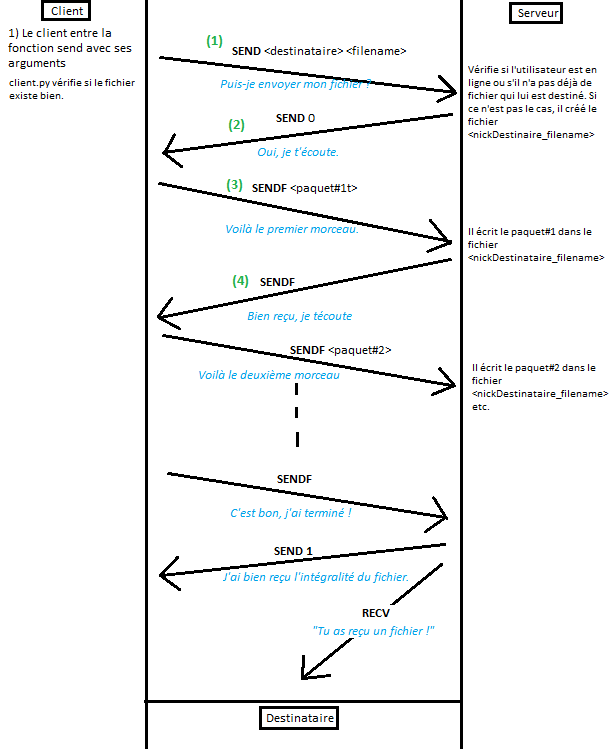
\includegraphics[height=15cm]{sendprotoc.png}

\end{document}

